\documentclass{report}

\usepackage[spanish]{babel}
\usepackage[utf8]{inputenc}
\usepackage{amssymb, amsmath}
\usepackage{graphicx}
\usepackage[left=20mm,right=20mm,top=20mm,bottom=20mm]{geometry}
\usepackage{gensymb}

\title{Tarea 4. Parámetros de PID método LGR}

\author{Miguel Hernández Umaña}

\begin{document}
\pagestyle{empty} 
\begin{center}
\textbf{{\Large Universidad de Costa Rica}\\}
\textbf{{\Large Facultad de Ingeniería}\\}
{\large Escuela de Ingeniería Eléctrica}\\
IE-0431 Sistemas de control\\
\vspace{60 mm}
Tarea 5. Diseño de controlador PID con LGR\\

\vfill
Estudiante: Miguel Hernández Umaña \\
Carnet: A42600\\
Grupo: 03\\



\thispagestyle{empty} 
\end{center}
 \newpage
\section*{Procesos a utilizar}
De acuerdo a las especificaciones dadas para obtener los parámetros del 
modelo de planta a utilizar en esta tarea, se tiene que para el carnet \textit{A42600}, 
se utiliza como base el carnet \textit{A42655} equivalente a \textit{Aapqmn}.

Planta para proceso subamortiguado con un cero:

\begin{equation*}
    P_{psubc}(s) = \frac{\beta(s+2)}{(s+1+\alpha j)(s+1-\alpha j)},\enskip \alpha = 0.1 \cdot max(p,q,m,n), \beta = 
    (0.1 \cdot min(p,q,m,n)+1)
\label{Eq:1}
\end{equation*}

Dado que el \(max(p,q,m,n) = 6\) y el \(min(p,q,m,n) = 2\), el modelo subamortiguado queda de la siguiente manera:

\begin{equation*}
    P_{psubc}(s) = \frac{1.2(s+2)}{(s+1+0.6 j)(s+1-0.6 j)} = \frac{1.2(s+2)}{s^2+2s+1.36} 
\label{Eq:2}
\end{equation*}

Planta Proceso Inestable:

\begin{equation*}
    P_{pi}(s) = \frac{\beta}{(s^2-\alpha)},\enskip \alpha = 0.1 \cdot max(p,q,m,n), \beta = (0.1 \cdot min(p,q,m,n)+1) 
\label{Eq:3}
\end{equation*}

Sustituyendo los valores de \(\alpha\) y \(\beta\) se tiene:

\begin{equation*}
    P_{pi}(s) = \frac{1.2}{(s^2-0.6)}
\label{Eq:4}
\end{equation*}

\section*{Ejercicio 1}

1.1) Determine los parámetros del controlador de la familia PID que sea más simple (P,
PD, PI, PID), tal que la respuesta del sistema de control a un cambio tipo escalón en el valor
deseado, tenga: tiempo de asentamiento al 2\% \(t_{a2} \leqslant 4\) segundos, un error permanente \(e_{pr0} \leqslant 
20\%\) y el menor sobrepaso máximo posible.\\

1.2) Determine los parámetros de un controlador de la familia PID (P, PD, PI, PID), tal que la respuesta del sistema de control a un cambio tipo escalón en el valor deseado, tenga: el
menor sobrepaso máximo posible, tiempo de asentamiento al 2\% \(t_{a2} \leqslant 4\) segundos y que la respuesta a un cambio escalón en la referencia y en la perturbación tenga error 
permanente cero.

El modelo de la planta a utilizar es:

\begin{equation*}
    P_{psubc}(s) = \frac{1.2(s+2)}{(s+1+0.6 j)(s+1-0.6 j)} = \frac{1.2(s+2)}{s^2+2s+1.36} 
\label{Eq:5}
\end{equation*}

\subsubsection{Controlador Proporcional P \(C(s) = K_p\)}
El sistema se puede comparar con el modelo de un sistema subamortiguado 

\begin{equation*}
    \frac{y(s)}{r(s)}=\frac{K_{yr}\omega_n^2}{s^2+2\zeta \omega_ns+\omega_n^2}
\label{Eq:6}
\end{equation*}

Comparando denominadores se tiene que \(\zeta \omega_n = 1\). Además, para el modelo subamortiguado el tiempo de 
asentamiento al 2\% \(t_{a2} \approx \frac{4}{\zeta \omega_n}\).\\

Por lo tanto, para el ejercicio, sustituyendo \(\zeta \omega_n = 1\) en \(4 \leqslant \frac{4}{\zeta \omega_n}\), se tiene 
que \(1 \leqslant \zeta \omega_n\) para garantizar el tiempo de asentamiento requerido.\\

Utilizando el requerimiento de que el error permanente \(e_{pr0} \leqslant 20\%\). El error permanente se obtiene de la 
expresión:

\begin{equation*}
    e_{pr0} = \frac{1}{1+K_0},\enskip donde \enskip K_0 = \lim_{s\to0} C(s)P(s) 
\label{E:7}
\end{equation*}

Por lo tanto \(\frac{1}{1+K_0} \leqslant 0.2\), de donde se obtiene \(4 \leqslant K_0\). Sustituyendo este valor \(K_0\) en 
el límite:

\begin{equation*}
    4 \leqslant K_0 = \lim_{s\to0} K_p\frac{1.2(s+2)}{s^2+2s+1.36} 
\label{E:8}
\end{equation*}

de donde se obtiene que \(2.27 \leqslant K_p\). \\

Con estas condiciones, se pueden asegurar los requerimientos del sistema utilizando el controlador más simple, ejercicio 1.1), en este 
caso uno proporcional. En la figura \ref{F:1} se aprecia que para una ganancia \(2.27 \leqslant K_p\) y un \(1 \leqslant 
\zeta \omega_n\), aseguramos un \(t_{a2} \leqslant 4\) segundos y un error permanente \(e_{pr0} \leqslant 20\% \). En este 
caso el sobrepaso máximo da como resultado un 4.02\%. De hecho, observando el límite que propone el tiempo de 
asentamiento requerido, este se cumple independientemente de la ganancia, ya que el LGR está en su totalidad a la 
izquierda del límite \(-\zeta \omega_n\).

\begin{figure}[h!]
\centering  
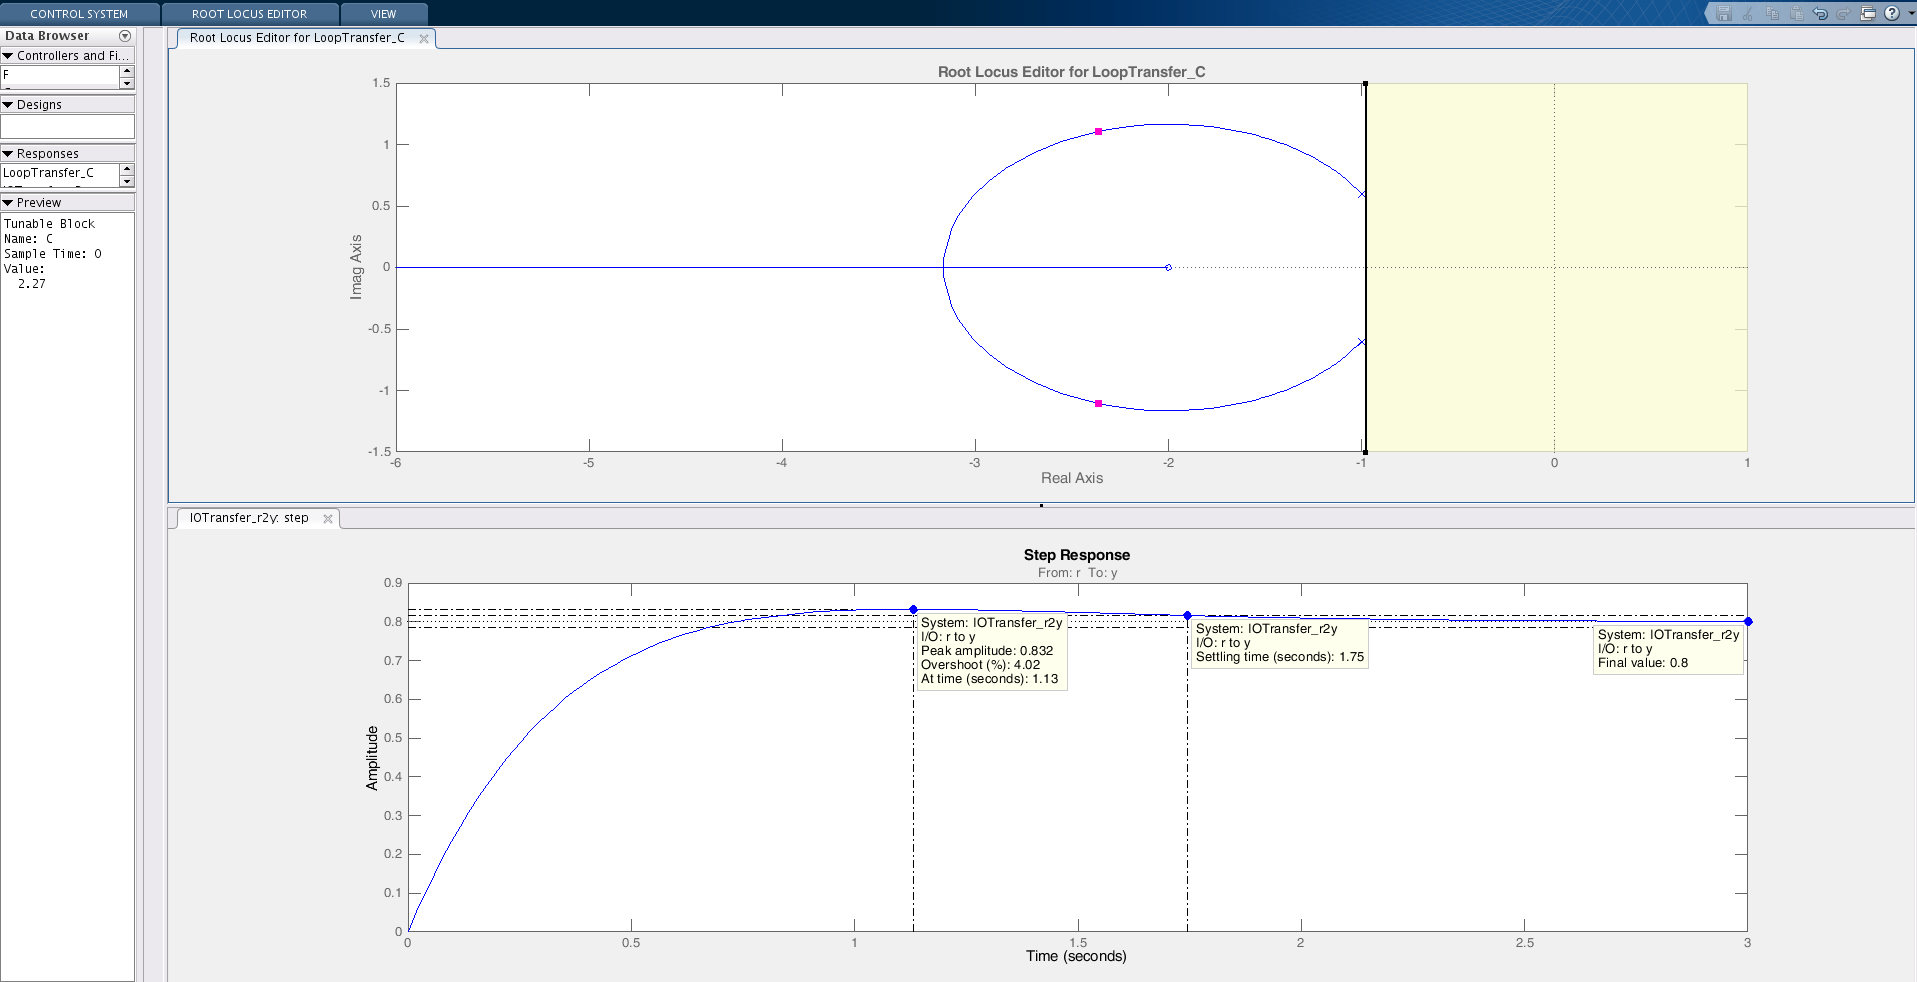
\includegraphics[width=1\textwidth]{P1_1.png}
\caption{Resultados para controlador proporcional \(K_p = 2.27\)}
\label{F:1}
\end{figure}

Aunque en la teoría el sobrepaso debería ser cero, acá se presenta este pequeño valor debido al cero que presenta el sistema en su función de transferencia. 

\subsubsection{Controlador Proporcional Derivativo PD \(C(s) = K_p(T_ds+1)\)}

Calculando el polinomio característico utilizando un controlador PD, se tiene:

\begin{equation*}
    1+C(s)P(s)= 1+ \frac{1.2K_p(s+2)(T_ds+1)}{s^2+2s+1.36} = ... = \frac{(1+1.2K_pT_d)s^2+(2+2.4K_pT_d+1.2K_p)s+(1.36+2.4K_p)}{s^2+2s+1.36}
    \label{Eq:12}
\end{equation*}

De los requerimientos, sabemos que \(2\zeta \omega_n = 2 \cdot 1 = 2\). Comparando con el polinomio obtenido usando el controlador PD y usando \(K_p = 2.77\) se tiene:

\begin{equation*}
    2\zeta \omega_n = 2 = 2+2.4K_pT_d+1.2K_p  \Leftrightarrow T_d = -0.5
\end{equation*}

En la figura \ref{F:P1_PD} se muestran los resultados dado este valor de \(T_d\). Sin embargo con este controlador no se logra obtener un error permanente cero por lo que se continúa calculando 
los resultados para los otros controladores.

\begin{figure}[h!]
    \centering  
    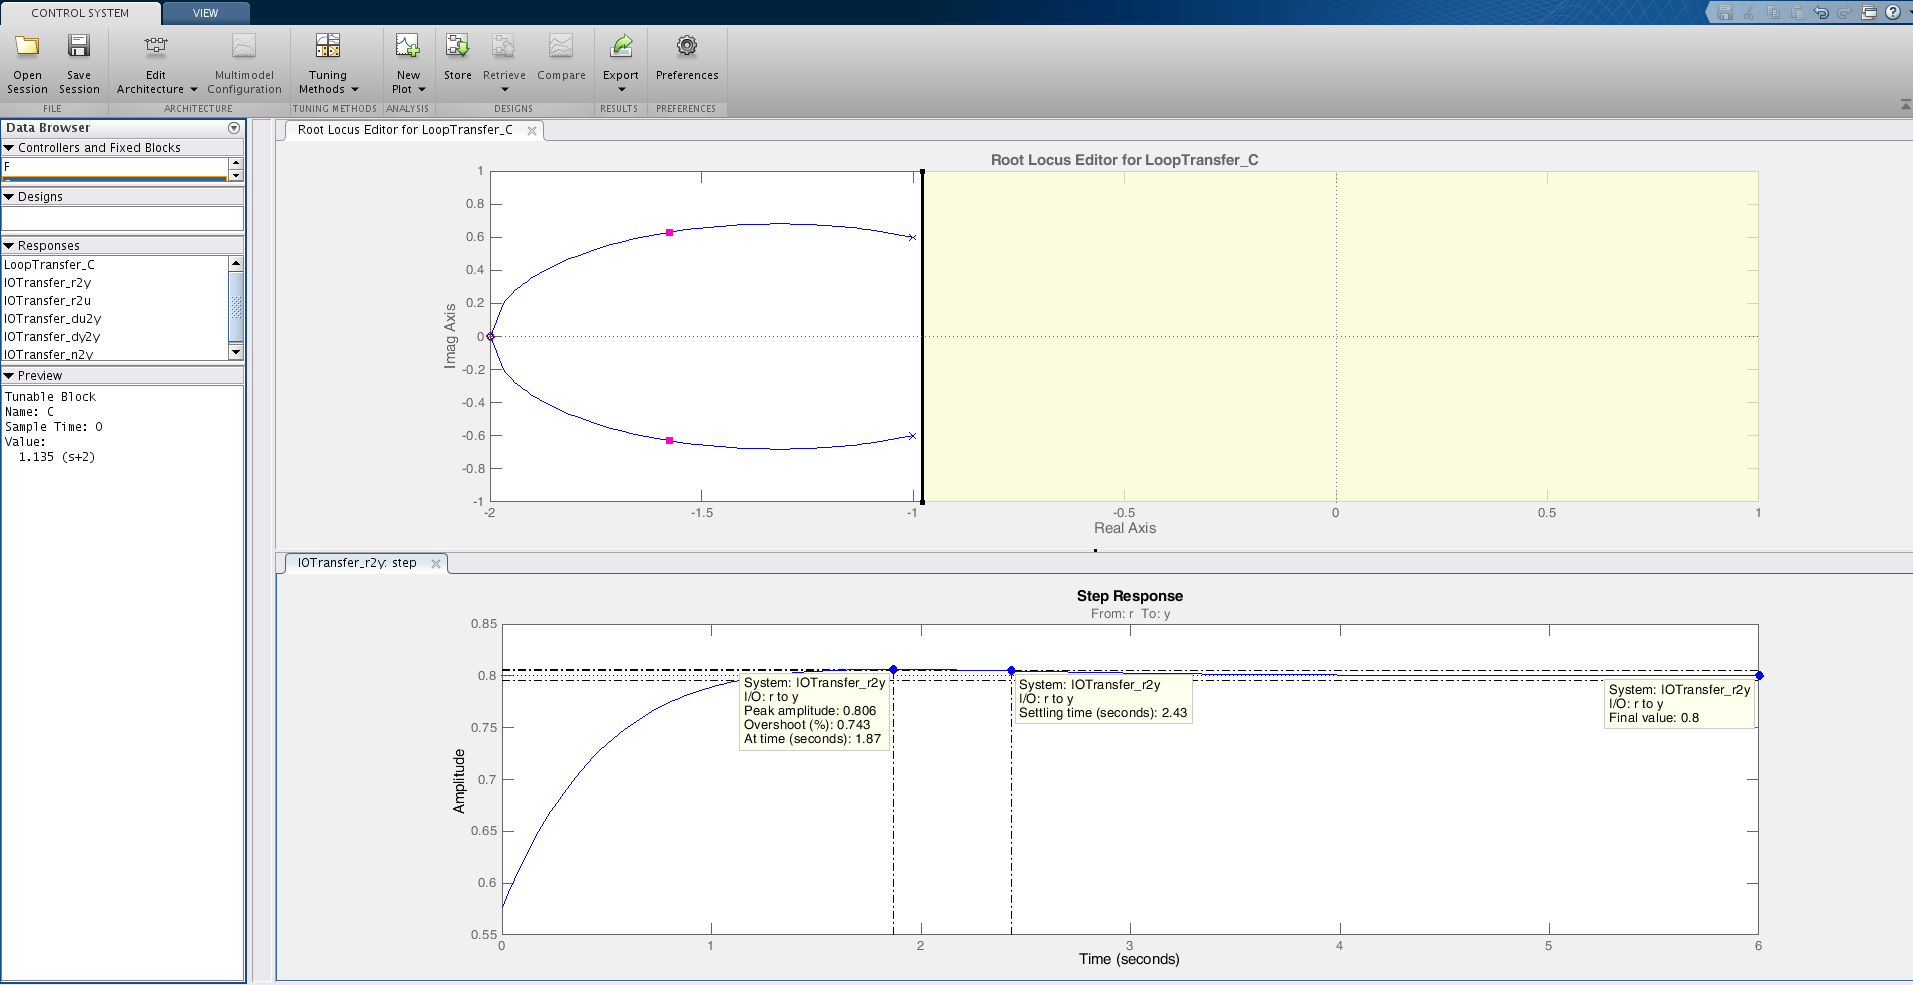
\includegraphics[width=1\textwidth]{P1_PD.png}
    \caption{Resultados para controlador PD}
    \label{F:P1_PD}
    \end{figure}

\subsubsection{Controlador Proporcional Integral PI \(C(s) = K_p \frac{T_is+1}{T_is}\)}
Utilizando el mismo valor que para el cero que el modelo con PD, pero agregando un polo en el origen, se obtiene el error permanente cero, \(T_i=0.5\). El polinomio característico se convierte en uno de orden 3
por lo que se utiliza el apoyo de la herramienta SISOTOOL para obtener el resultado gráficamente y verificar que se cumplen los requerimientos.

\begin{equation*}
    1+C(s)P(s)= 1+ \frac{1.2K_p(s+2)T_i(s+1/T_i)}{T_is(s^2+2s+1.36)} = ... = \frac{s^3+3.2s^2+(3.76+1.2/T_i)s+(2.4/T_i)}{s(s^2+2s+1.36)}
    \label{Eq:12}
\end{equation*}

donde el polinomio característico es \(p.c = s^3+3.2s^2+(3.76+1.2/T_i)s+(2.4/T_i)\).\\

De la herrramienta en Matlab se obtiene la figura \ref{F:P1_PI}.\\

\begin{figure}[h!]
    \centering  
    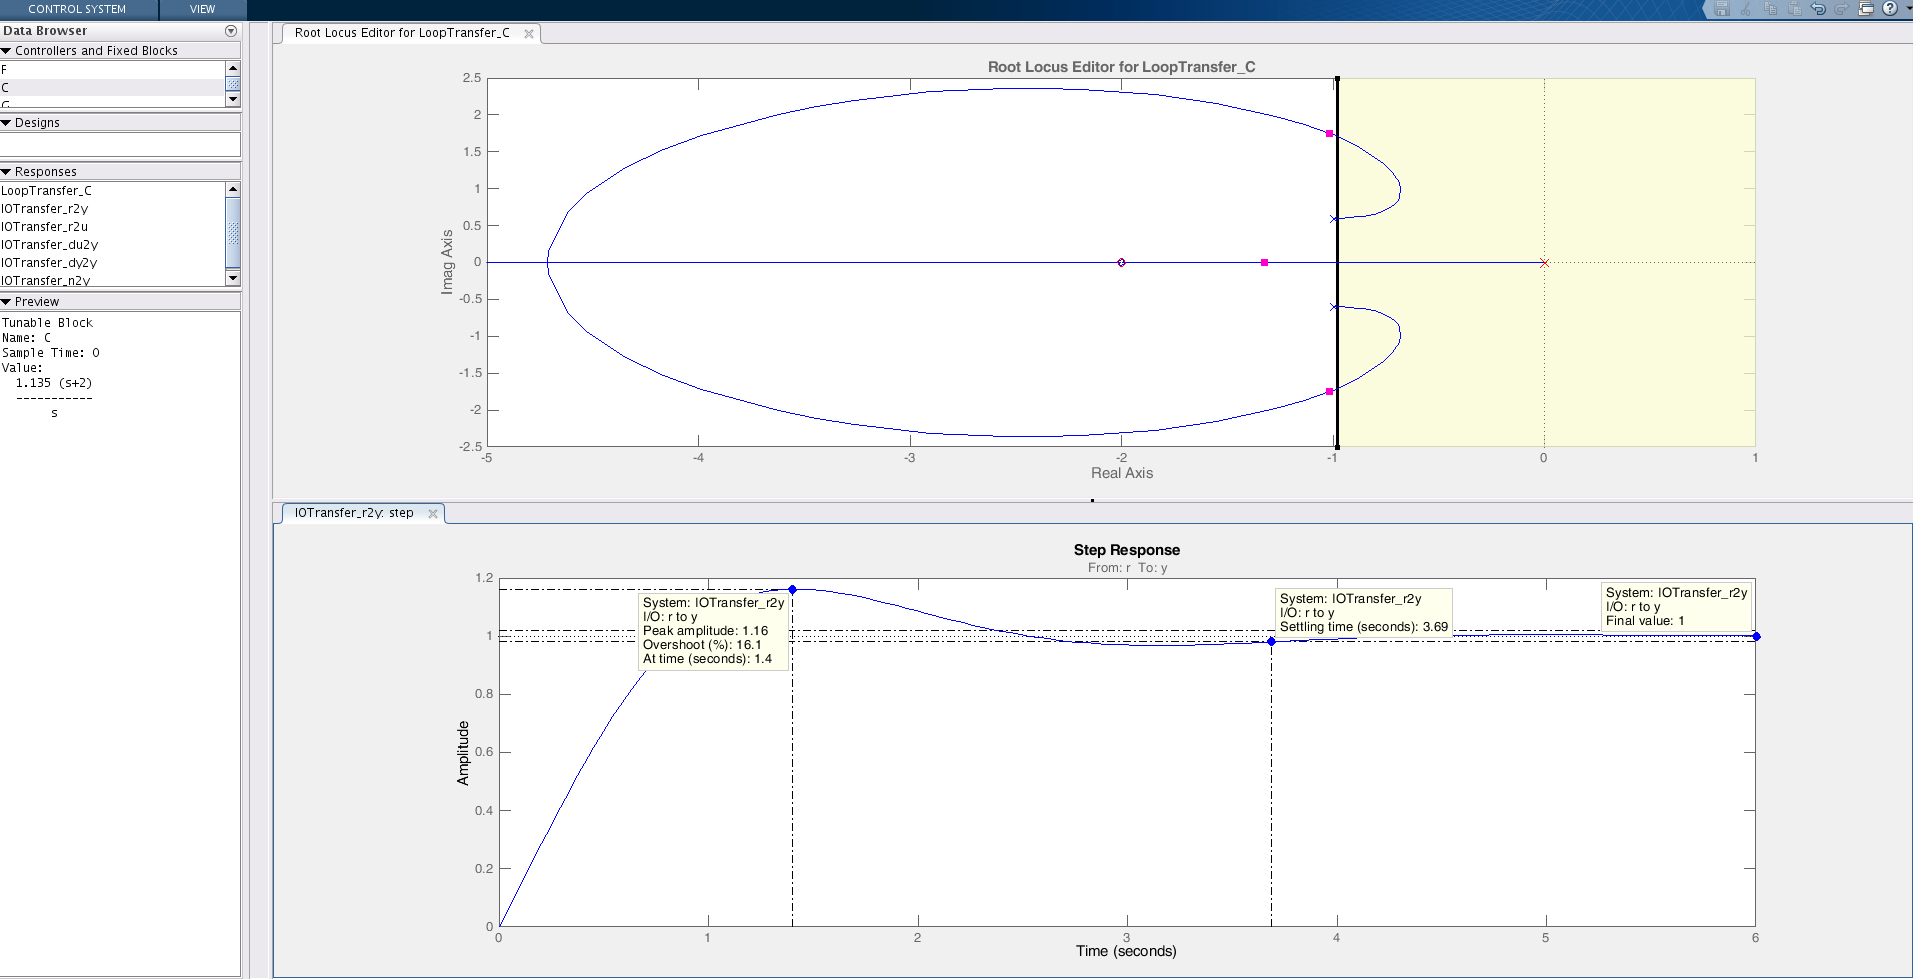
\includegraphics[width=1\textwidth]{P1_PI.png}
    \caption{Resultados para controlador PI}
    \label{F:P1_PI}
\end{figure}

Se observa que con el controlador PI indicado se cumplen los requerimientos solicitados en el ejercicio 2.2), los cuales son el más bajo sobrepaso máximo, \(t_{a2} \leqslant 4\) y error permanente cero.
%%%%%%%%%%%%%%%%%%%%%%%%%%%%%%%%% EJERCICIO 2 %%%%%%%%%%%%%%%%%%%%%%%%%%%%%%%%%%%%
\section*{Ejercicio 2}
Para el proceso representado por el modelo personalizado inestable \(P_{pi}(s)\):
Se desea que la respuesta del sistema de control, a un cambio tipo escalón en el valor deseado, tenga las siguientes características: sobrepaso máximo \(M_{pn\%} = 16.3\%\) y un tiempo de 
asentamiento al 2\% \(t_{a2\%} \leqslant 4,0\) s.\\

2.1) Determine los parámetros del controlador de la familia PID más simple posible (P, PD, PI, PID), que permite cumplir con las especificaciones deseadas. Indique y justifique
claramente cuáles de las especificaciones se pueden cumplir y cuáles no, para cada tipo de controlador analizado. Indique claramente los valores de las especificaciones 
(\(M_{pn\%}, t_{a2\%}\)) obtenidas únicamente para el controlador seleccionado, además del valor del \(e_{pr0}\).\\

2.2) Considerando que ahora se desea un \(e_{pr0}=0\%\), determine los parámetros del controlador de la familia PID más simple posible (P, PD, PI, PID), que permite cumplir con todas
las especificaciones. Indique y justifique claramente cuáles de las especificaciones se pueden cumplir y cuáles no, para cada tipo de controlador analizado. Indique claramente los valores de
las especificaciones (\(M_{pn\%}, t_{a2\%}\) y \(e_{pr0}\)) únicamente para el controlador seleccionado.

\subsubsection{Controlador Proporcional P \(C(s) = K_p\)}

Considerando el proceso inestable:
\begin{equation*}
    P_{pi}(s) = \frac{1.2}{(s^2-0.6)} = \frac{1.2}{(s-0.7746)(s+0.7746)} 
\label{Eq:9}
\end{equation*}

Se comienza el análisis calculando el polinomio característico deseado. De la expresión \(M_{pn\%} = 16.3\% = e^\frac{\zeta \pi}{\sqrt{1-\zeta ^2}}\) se obtiene que \(\zeta \approx 0.5\). Luego, 
\(\theta = \cos^{-1}(\zeta) = 60^{\circ}\).

Del requerimiento \(t_{a2\%} = \frac{4}{\zeta \omega_n} \leqslant 4,0\), se obtiene que \(1 \leqslant \zeta \omega_n\). Se conoce \(\zeta = 0.5\), por lo que \(\omega_n = 2\). Con estos datos 
se construye el polinomio característico deseado.

\begin{equation*}
    p.c.deseado(s) = s^2+2\zeta \omega_n + \omega_n^2 = s^2+2s+4 
\label{Eq:10}
\end{equation*}

Se calcula el polinomio característico a partir de la aplicación del controlador proporcional \\

\begin{equation*}
    1 + C(s)P(s) =  1 + \frac{1.2 K_p}{s^2-0.6} = \frac{s^2-0.6 + 1.2 K_p}{s^2-0.6} \Leftrightarrow p.c = s^2-0.6 + 1.2 K_p
    \label{Eq:11}
\end{equation*}


Si se comparan los polinomios característicos, es evidente que son diferentes y no se pueden igualar. El polinomio obtenido usando el controlador proporcional no posee el término que depende de 
de \(\zeta \omega_n\). Gráficamente esto indica que la línea límite \(\zeta \omega_n = 0\) o que está sobre el eje Y, como se observa en la figura \ref{F:P2_P}. O sea, no se podrán cumplir ninguno de los requerimientos solicitados ya que 
el sistema es inestable.

\begin{equation*}
    p.c.deseado(s) \neq p.c.obtenido \Leftrightarrow s^2+2s+4 \neq s^2-0.6 + 1.2 K_p
\label{Eq:12}
\end{equation*}

\begin{figure}[h!]
    \centering  
    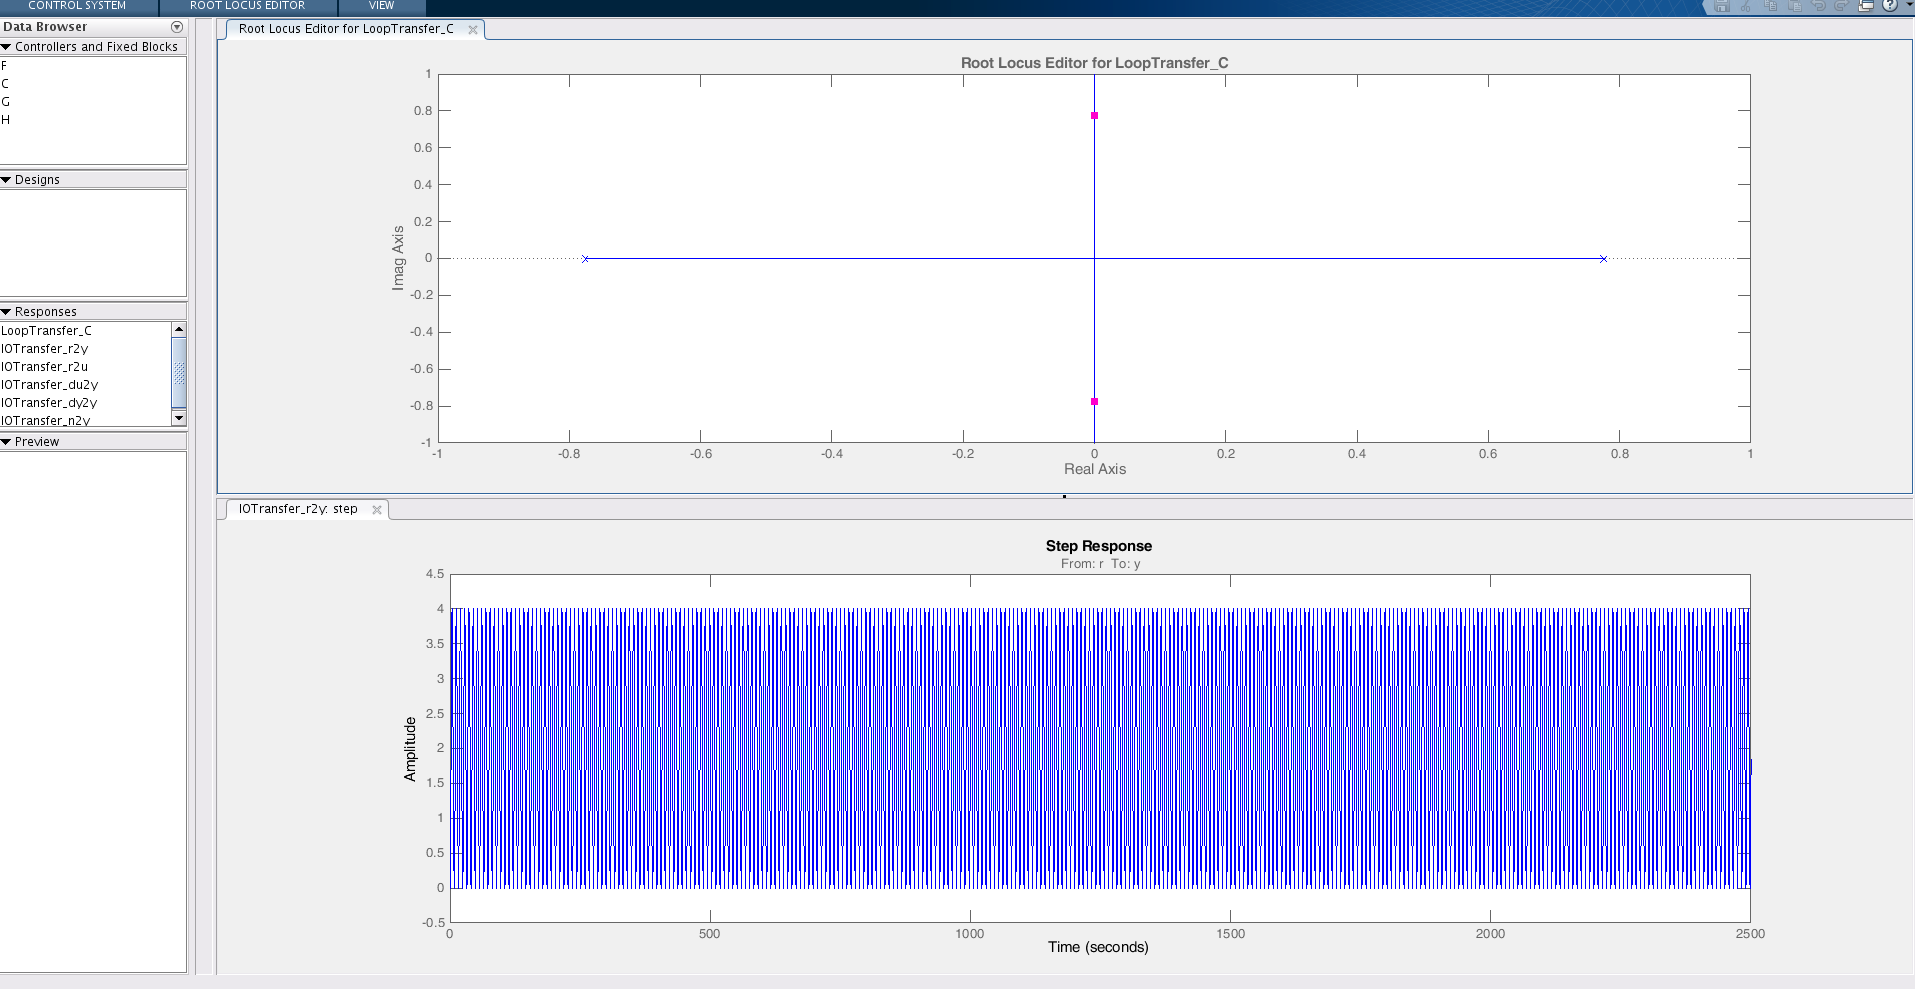
\includegraphics[width=1\textwidth]{P2_P.png}
    \caption{Resultados para controlador proporcional en sistema inestable}
    \label{F:P2_P}
\end{figure}

\subsubsection{Controlador Proporcional Derivativo PD \(C(s) = K_p(T_ds+1)\)}

Ahora se generan los cálculos utilizando un controlador PD. \\

El polinomio característico en este caso será:

\begin{equation*}
    1+C(s)P(s)= 1+ \frac{1.2K_p(T_ds+1)}{s^2-0.6} \Leftrightarrow p.c. = s^2+(1.2K_pT_d)s+(1.2K_p-0.6)
    \label{Eq:12}
\end{equation*}


Este polinomio característico sí es comparable con el polinomio característico deseado. Se plantea el sistema de ecuaciones:


\begin{eqnarray*}
    1.2K_pT_d  = 2 \\
    1.2K_p-0.6 = 4 \\
\end{eqnarray*}

Del cual se obtiene \(K_p = \frac{23}{6} \approx 3.833\) y \(Td = \frac{10}{23} \approx 0.435\).\\

Con estos valores se tienen los siguientes valores para los requerimientos:\\

\(M_{pn\%} = 16.3\%\), \(t_{a2\%} \leqslant 4,0 \) y \(e_{pr0}=-15\%\) (el negativo indica que el valor final está sobre el valor deseado).\\

En la figura \ref{F:P2_PD} se presentan los resultados, con lo cual con este controlador PD se cumplen los requerimientos del ejercicio 2.1). Se deben considerar las diferencias que se obtienen entre los valores calculados con los dados por SISOTOOL, en los primeros las ecuaciones utilizadas 
son aproximaciones y los resultados de Matlab contienen otra precisión. La mayor diferencia se presenta en el sobrepaso máximo donde SISOTOOL arroja 26.2\%, en parte también debido al cero que agrega 
el controlador PD.

\begin{figure}[h!]
    \centering  
    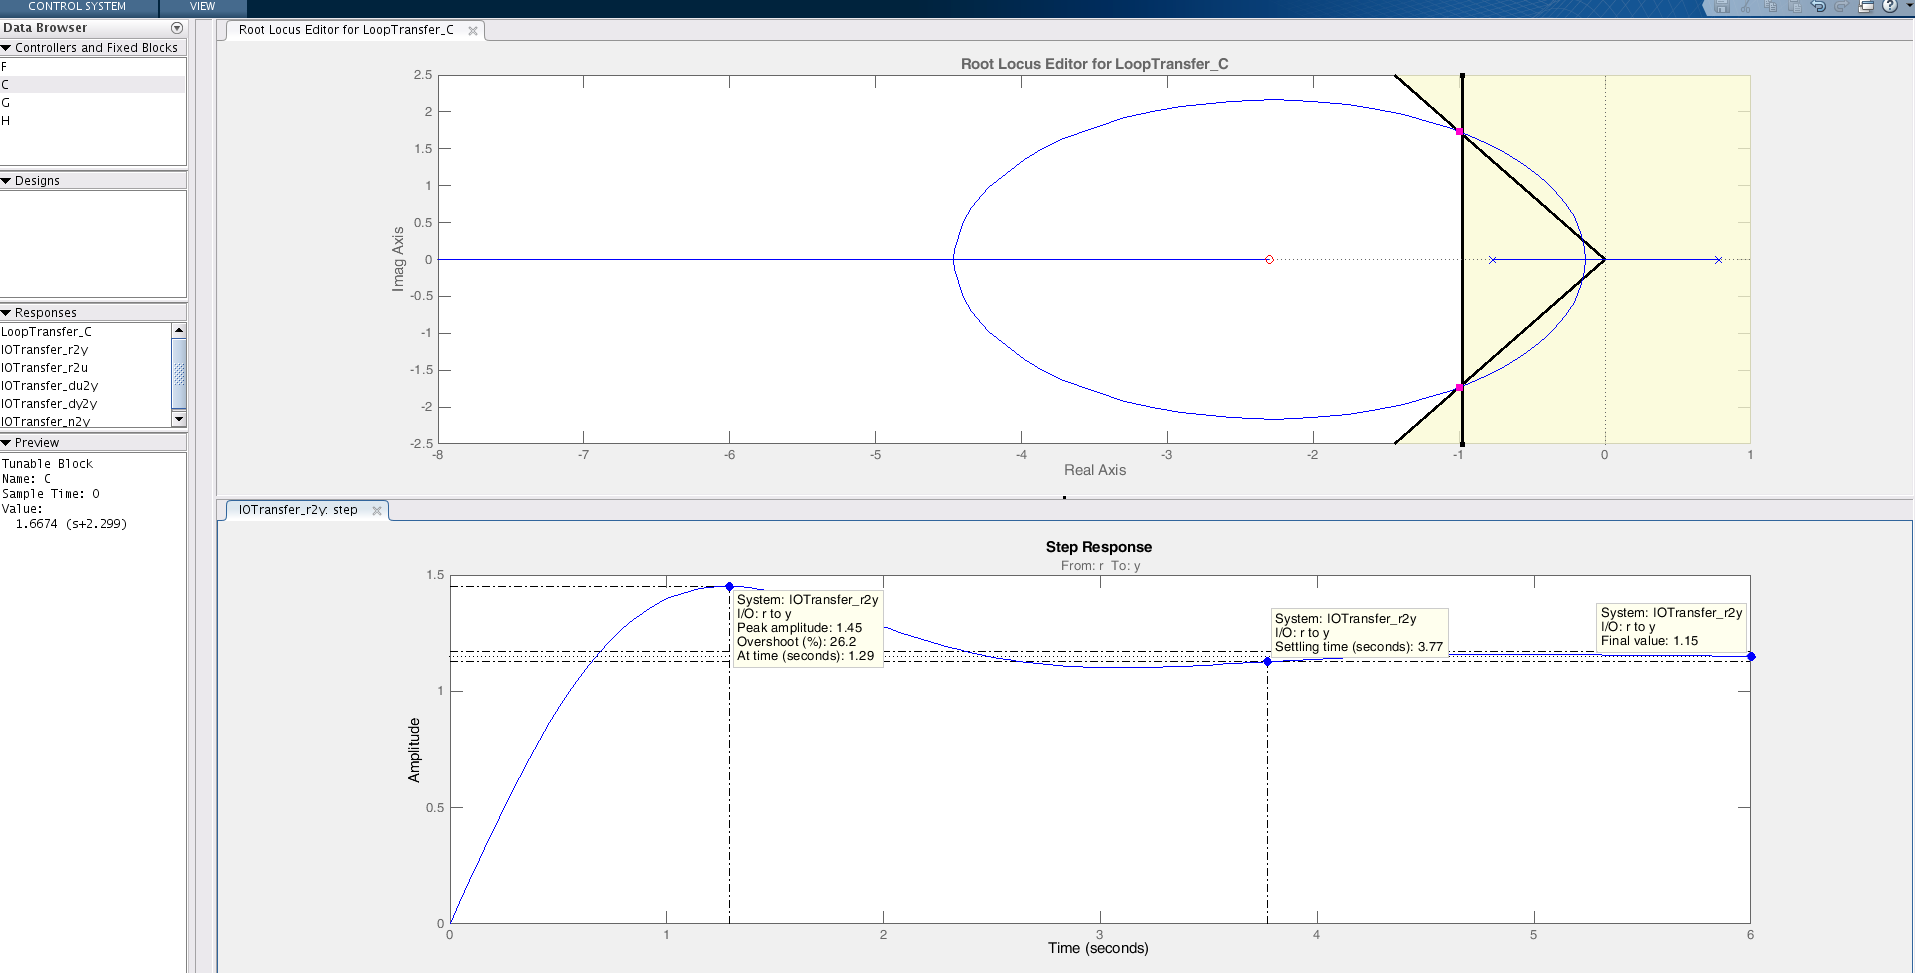
\includegraphics[width=1\textwidth]{P2_PD.png}
    \caption{Resultados para controlador proporcional derivativo en sistema inestable}
    \label{F:P2_PD}
\end{figure}

\subsubsection{Controlador Proporcional Integral PI \(C(s) = K_p \frac{T_is+1}{T_is}\)}

Se calcula el polinomio característico utilizando el Controlador Proporcional Integral.\\

\begin{equation*}
    1+C(s)P(s)= 1 + \frac{1.2K_p(T_is+1)}{T_is(s^2-0.6)} = 1 + \frac{1.2K_pT_i(s+1/T_i)}{T_is(s+\sqrt{15}/5)(s-\sqrt{15}/5)}
    \label{Eq:13}
\end{equation*}

Se busca un valor para \(1/T_i\) de manera tal que cancele el polo inestable del sistema. Por lo tanto \(1/T_i=-\sqrt{15}/5\), lo cual permite simplificar la expresión a:

\begin{equation*}
    1+C(s)P(s) =  1 + \frac{1.2K_p}{s(s+\sqrt{15}/5)} \Leftrightarrow p.c. = s^2+\sqrt{15}/5s+1.2K_p
    \label{Eq:14}
\end{equation*}

Este polinomio característico no es comparable con el polinomio característico deseado, por lo que se presenta un polinomio característico factible, que permitirá cumplir algunos de los
requerimientos del ejercicio, en este caso el de sobrepaso máximo.\\

Como se cancela el polo inestable y se agrega un polo en el el origen, el integrador, ahora el LGR cambia y las ramas salen del punto medio entre 0 y \(-\sqrt{15}/5\), que es \(-\sqrt{15}/10\). 
En la figura \ref{F:P2_PI} se muestra el LGR resultante. De acá se observa que el sistema no es capaz de cumplir el tiempo de asentamiento, deteminado por la recta vertical \(\zeta \omega_n \approx -1\).

\begin{figure}[h!]
    \centering  
    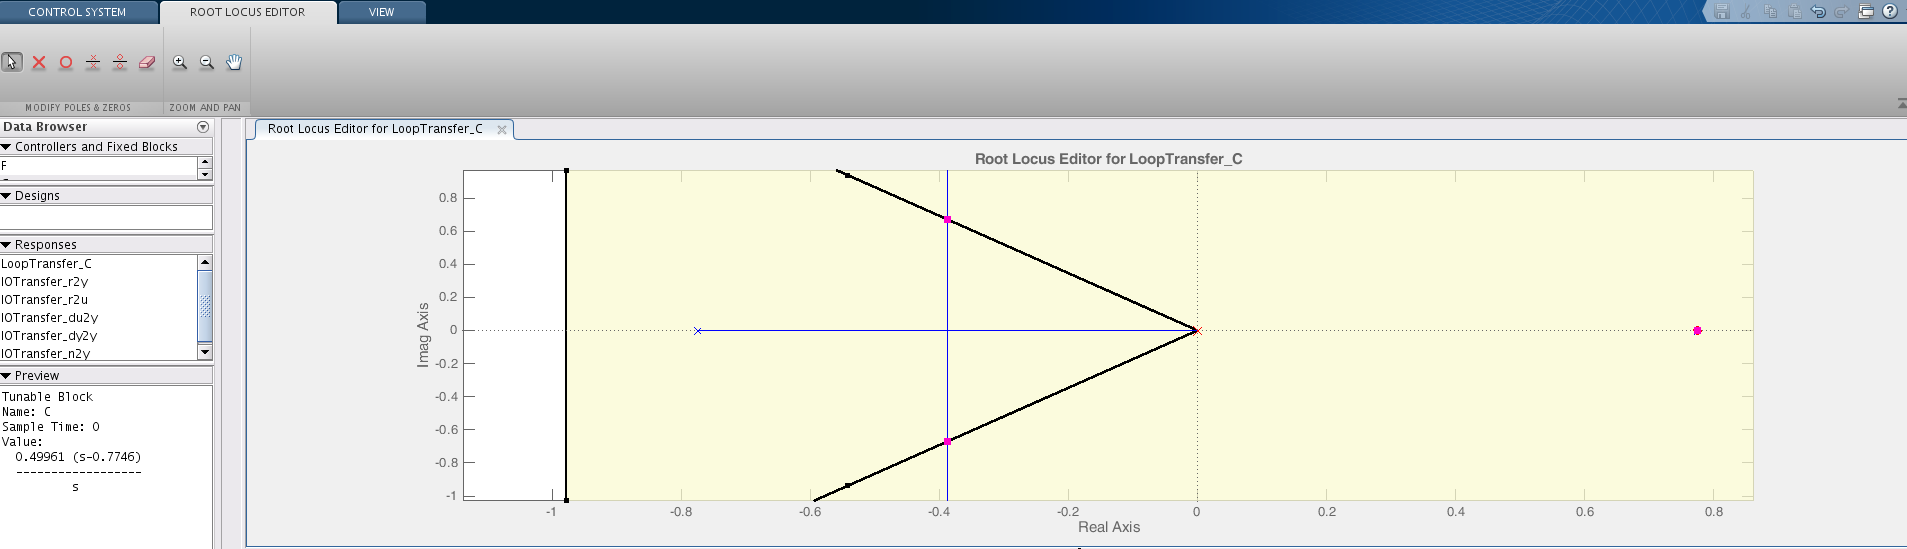
\includegraphics[width=1\textwidth]{P2_PI.png}
    \caption{Resultados para controlador proporcional integrador en sistema inestable}
    \label{F:P2_PI}
\end{figure}

Nota: SISOTOOL no muestra correctamente, por algún tipo de error, la gráfica temporal.\\

Para calcular el punto de intersección entra el nuevo LGR y las rectas límite del tiempo de asentamiento, se tiene el valor real \(\sqrt{15}/10\); con trigonometría se calcula el valor imaginario.\\


\begin{equation*}
    \tan(\theta) = \frac{Im}{Re} \Leftrightarrow \tan(60) = \frac{Im}{\sqrt{15}/10} \Leftrightarrow Im = 3\sqrt{5}/10 \approx 0.67
    \label{Eq:15}
\end{equation*}



Por lo que los factores del p.c.factible son \((s+\sqrt{15}/10-3\sqrt{5}/10 i)(s+\sqrt{15}/10+3\sqrt{5}/10 i) \). El polinomio es \(s^2+\sqrt{15}/5s+3/5\).\\

Este polinomio factible sí es comparable con el obtenido con el controlador PI. Comparándolos se obtiene que \(1.2K_p=3/5 \Leftrightarrow K_p = 0.5 \).\\

Para este polinomio se tienen los siguientes valores para los requerimientos:\\

\(M_{pn\%} = 16.3\%\), \(t_{a2\%} = \frac{4}{\zeta \omega_n} = \frac{4}{\sqrt{15}/10} \approx 10.33 \), lejos del requerido y \(e_{pr1}=0\%\) debido al integrador.\\


\subsubsection{Controlador Proporcional Integral Derivativo PID \(C(s) = K_p (T_ds+1)\frac{T_is+1}{T_is}\)}

Se mantiene el valor de \(T_i = -\sqrt{15}/3 \approx -1.29\) para cancelar el polo inestable.\\

Se calcula el polinomio característico para el controlador PID:

\begin{equation*}
    1 + \frac{1.2K_p(T_ds+1)T_i(s-1/T_i)}{T_is(s-\sqrt{15}/5)(s+\sqrt{15}/5)} = 1+ \frac{1.2K_p(T_ds+1)}{s(s+\sqrt{15}/5)} = \frac{s^2+(\sqrt{15}/5+1.2K_pT_d)s+(1.2K_p)}{s(s+\sqrt{15}/5)}
\end{equation*}

Igualando polinomios característicos \(s^2+(\sqrt{15}/5+1.2K_pT_d)s+(1.2K_p) = s^2+2s+4\), obteniendo el sistema de ecuaciones:

\begin{eqnarray*}
    \sqrt{15}/5+1.2K_pT_d  = 2 \\
    1.2K_p = 4 \\
\end{eqnarray*}

Resolviendo, se obtienen los valores \(K_p=10/3 \approx 3.33\) y \(T_d = (10-\sqrt{15})/20 \approx 0.306\).\\

El resultado obtenido con estos parámetros se muestra en la figura \ref{F:P2_PID}.\\

\begin{figure}[h!]
    \centering  
    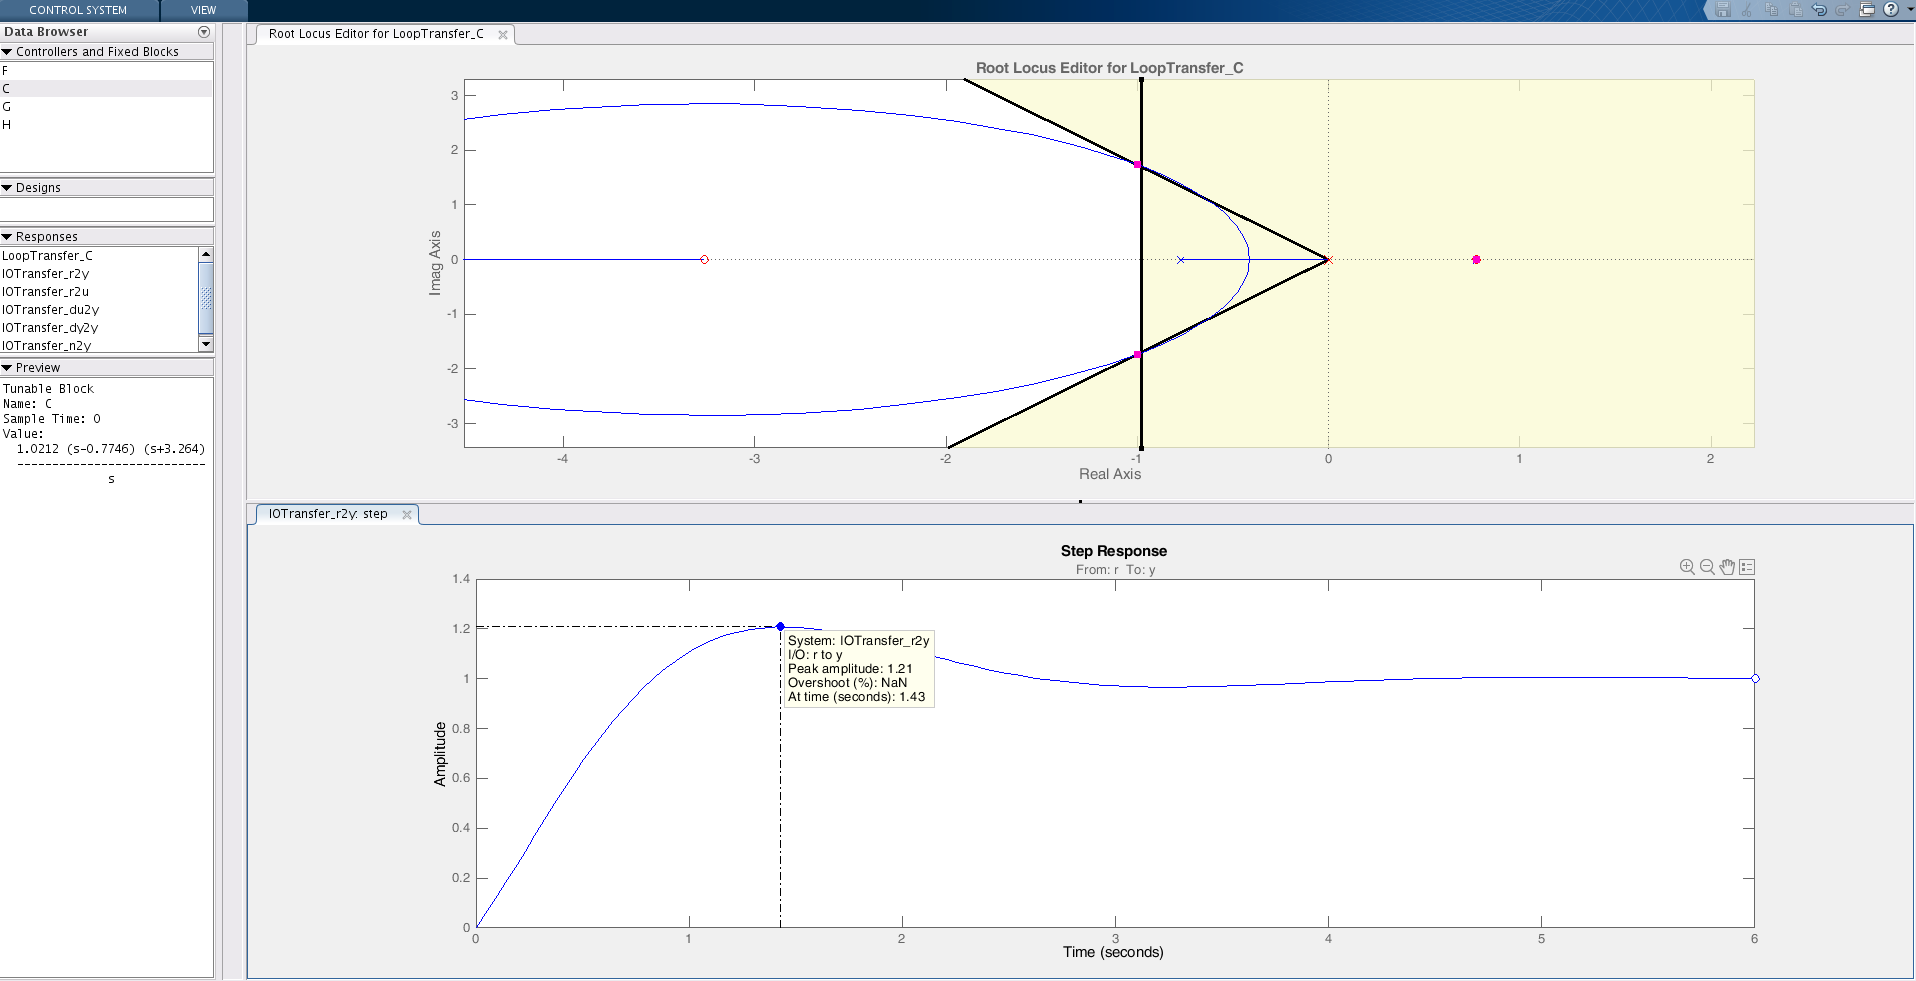
\includegraphics[width=1\textwidth]{P2_PID.png}
    \caption{Resultados para controlador PID en sistema inestable}
    \label{F:P2_PID}
\end{figure}

Así, con estos valores se obtienen los requerimientos dados: \(M_{pn\%} = 16.3\%\), \(t_{a2\%} \leqslant 4,0\) y \(e_{pr0}=0\), siendo estos los requeridos por el ejercicio 2.2)\\

Nota: SISOTOOL no muestra, por algún tipo de error, los datos de tiempo de asentamiento y valor final.





\end{document}